\section{Background and Motivation}

\subsection{Context Adaptation}

Context adaptation (or context engineering) refers to methods that improve model behavior by constructing or modifying inputs to an LLM, rather than altering its weights.
The current state of the art leverages \textit{natural language feedback}~\citep{shinn2023reflexion, yuksekgonul2024textgrad, agrawal2025gepa}.
In this paradigm, a language model inspects the current context along with signals such as execution traces, reasoning steps, or validation results, and generates natural language feedback on how the context should be revised.
This feedback is then incorporated into the context, enabling iterative adaptation.
Representative methods include Reflexion~\citep{shinn2023reflexion}, which reflects on failures to improve agent planning; TextGrad~\citep{yuksekgonul2024textgrad}, which optimizes prompts via gradient-like textual feedback; 
GEPA~\citep{agrawal2025gepa}, which refines prompts iteratively based on execution traces and achieves strong performance, even surpassing reinforcement learning approaches in some settings;
and Dynamic Cheatsheet~\citep{krause2019dynamic}, which constructs an external memory that accumulates strategies and lessons from past successes and failures during inference.
These natural language feedback methods represent a major advance, offering flexible and interpretable signals for improving LLM systems beyond weight updates.

\subsection{Limitations of Existing Context Adaptation Methods}
\label{subsec:limitations}

\paragraph{Brevity Bias}
A recurring limitation of context adaptation methods is \textit{brevity bias}: the tendency of optimization to collapse toward short, generic prompts.
Gao et al.~\citep{gao2025prompt} document this effect in prompt optimization for test generation, where iterative methods repeatedly produced near-identical instructions (\eg, “Create unit tests to ensure methods behave as expected”), sacrificing diversity and omitting domain-specific detail.
This convergence not only narrows the search space but also propagates recurring errors across iterations, since optimized prompts often inherit the same faults as their seeds.
More broadly, such bias undermines performance in domains that demand detailed, context-rich guidance—such as multi-step agents, program synthesis, or knowledge-intensive reasoning—where success hinges on accumulating rather than compressing task-specific insights.

\begin{figure}[htbp]
    \centering
    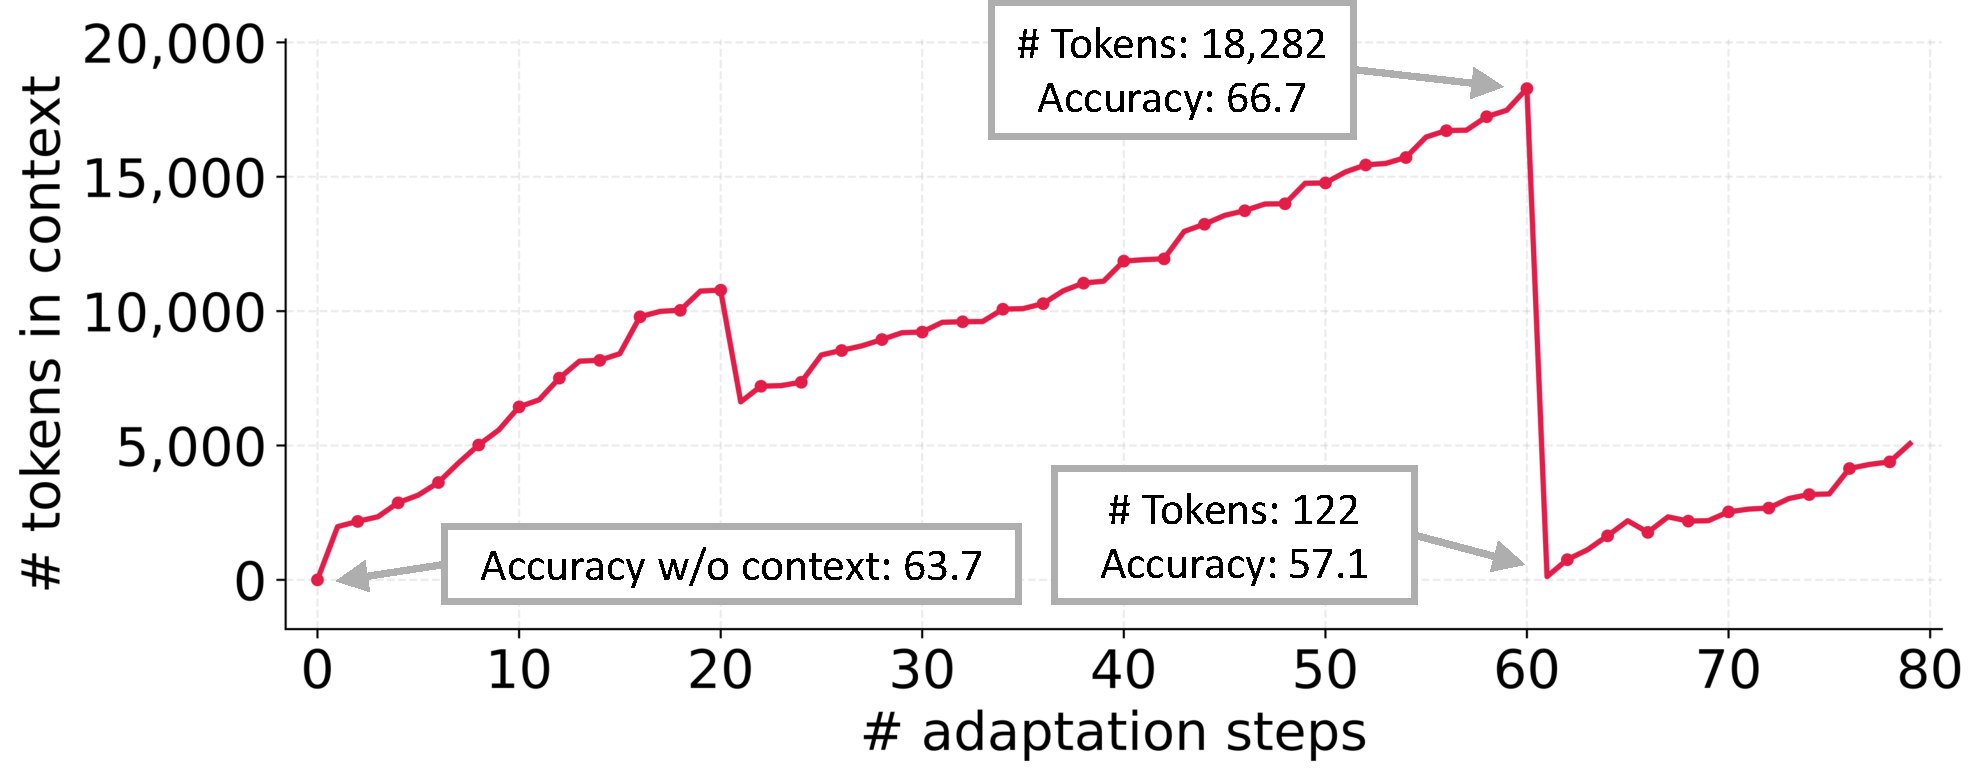
\includegraphics[width=0.8\textwidth]{figures/figure_2_CR.pdf}
    \caption{\textbf{Context Collapse.} Monolithic rewriting of context by an LLM can collapse it into shorter, less informative summaries, leading to sharp performance drops. }
    \label{fig:context-collapse}
\end{figure}

\paragraph{Context Collapse} 
In a case study on the AppWorld benchmark~\citep{trivedi2024appworld}, we observe a phenomenon we call \textit{context collapse}, which arises when an LLM is tasked with fully rewriting the accumulated context at each adaptation step. 
As the context grows large, the model tends to compress it into much shorter, less informative summaries, causing a dramatic loss of information. 
For instance, at step 60 the context contained 18,282 tokens and achieved an accuracy of 66.7, but at the very next step it collapsed to just 122 tokens, with accuracy dropping to 57.1—worse than the baseline accuracy of 63.7 without adaptation. 
While we highlight this through Dynamic Cheatsheet~\citep{suzgun2025dynamic}, the issue is not specific to that method; rather, it reflects a fundamental risk of end-to-end context rewriting with LLMs, where accumulated knowledge can be abruptly erased instead of preserved.

\begin{figure}[htbp]
    \centering
    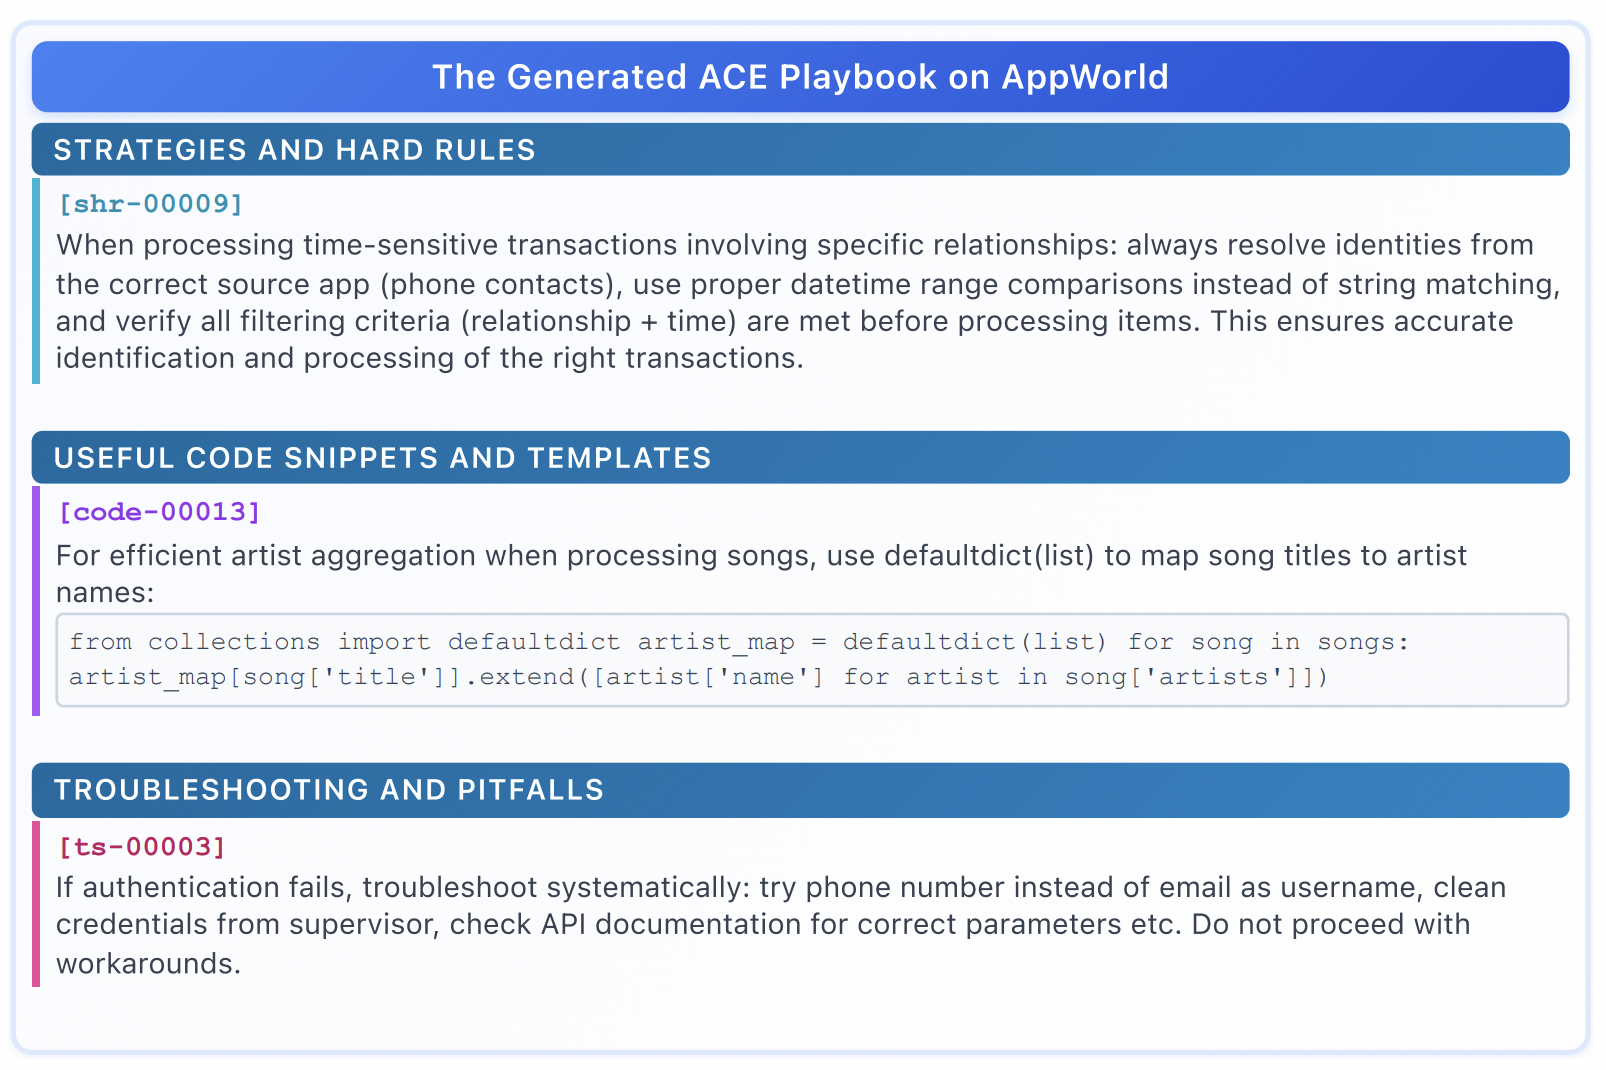
\includegraphics[width=0.9\textwidth]{figures/figure_3_CR.png}
    \caption{\textbf{Example ACE-Generated Context on the AppWorld Benchmark} (partially shown). ACE-generated contexts contain detailed, domain-specific insights along with tools and code that are readily usable, serving as a comprehensive playbook for LLM applications.}
\label{fig:ace-context-appworld-motivation}
\end{figure}